%\addcontentsline{toc}{chapter}{Development Process}
\chapter{Design}

\section{Overall Architecture}

The overall architecture of the project consists of a dynamic webpage with scripting to process user input and display back the results. The webpage has a form for the user to enter the SQL text and here the input SQL is parsed by the JavaScript code. The system attempts to build a database from the user input and if it succeeds it will display the database as a collection of tables back to the user. If the system fails to build the database it means that the SQL that the user entered has some syntax errors and can not be visualised. Once the database has been visualised then the user can also interact with the database by viewing the syntax highlighting of the SQL text and also viewing the list of flaws of the database.

\subsection{Consideration of Other Designs}

During the research stage of the project the aim was to find a third-party library that would handle SQL parsing so that this project could focus more on the visualising and structuring of the output. However this proved to not be possible since there were no open-source libraries that were available to parse the SQL and create some object that could be used to visualise the parsed database. Since this was not possible the main goal of this project was to create an SQL parser that would be able to check if the SQL compiles and if there were any syntax errors in the input.

Another design that was considered comprised of assuming that the user inserted SQL that compiles and has no syntax errors, this SQL would be for example exported from a database management system. This would make parsing easier since syntax error detection would not have to be implemented and instead the parser could include more syntax from the documentation and more time could be allocated to detection of more sophisticated flaw detection like normalisation. However the decision was made to instead focus on syntax error detection and include it in the parser since this project is aimed at SQL learners which means they are more likely to enter SQL with syntax errors.

\section{Code Structure}

The code is structured into classes that follow the data model of a database, this approach uses an object orientated approach using JavaScript ES6 classes. The classes are closely related to the properties of the PostgreSQL database, this means that a created database object will contains schemas, tables and columns just like a PostgreSQL database. This approach was taken to be able to create a "database" object and from there be able to visualise that object, which improves readability of the code base. The syntax errors in the SQL are also implemented in the JavaScript code as an error that is thrown when the database object could not be created due to syntax errors in the SQL input. This allows the creation of alerts to inform the user of the syntax error, the message in the error is displayed to the user in the alert.  
% elaborate more on the syntax error alerts

\newpage

\subsection{Class Diagram}

\begin{figure}[h!]
	\centering
	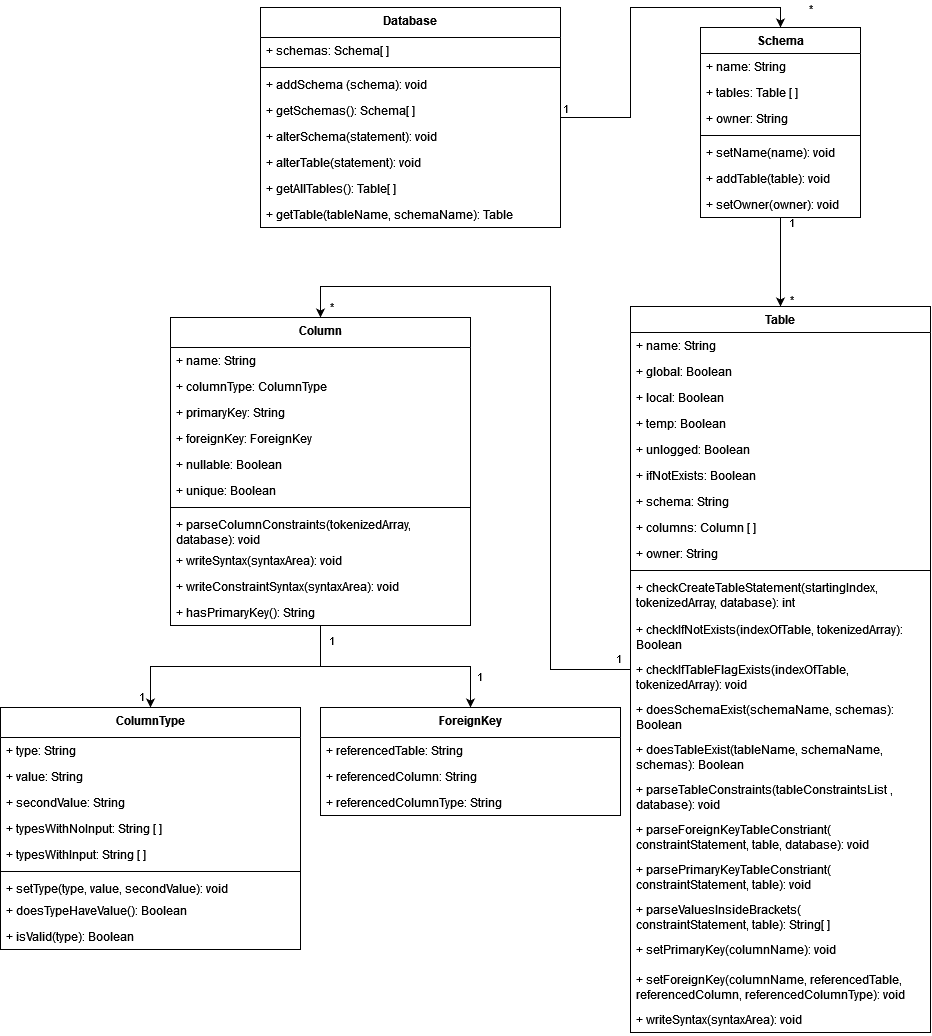
\includegraphics[width=\textwidth]{classDiagram}
	\caption{UML Class diagram for the project created using \cite{dbdiagram}}
	\label{fig:classDiagram}
\end{figure}

\newpage

\section{Algorithms}

\subsection{Parser}

As mentioned in the first chapter, the parser consists of a tokeniser and the proper parsing. To tokenise the input text a library was used \cite{tokeniser}, it is designed to turn JavaScript code into tokens however for the purpose of parsing SQL it is also appropriate. The library is powered by regular expressions and it almost complies with parsing specification. This library was chosen because of the token object it produces are easy to work with and the types of tokens are compatible with SQL and the parsing that was designed. The library consisted of an function that converted a string to token objects that were later converted into an array. The Token objects contained a type of token as well as the value of the token. This made parsing easier since after tokenising the input text, all white spaces could be ignored and each token would either be of type "Punctuator" or "IdentifierName". This meant that the array of values to parse only contained words or flags of SQL statements which were separated by punctuators which were used to identify the different syntax of each statement.

After the input has been tokenised the proper parsing has to be done to make sense of the SQL and check if there are syntax errors. This is achieved using regular expressions and further proper parsing. The regular expressions were created to match simple patterns in the SQL syntax, an example of this includes separating each SQL statement by a semicolon. Another example of this is separating each column in a "CREATE TABLE" statement. Each column should be separated by a comma, however commas are also present when a primary key is created with more than one column. To achieve this a regular expression was constructed to use Lookahead and Lookbehind was used to see if the comma is surrounded by brackets and not match that comma.

\begin{figure}[h!]
	\centering
	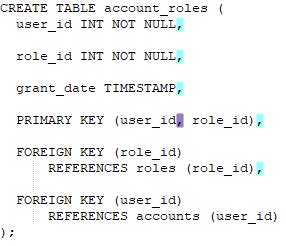
\includegraphics{regex}
	\caption{Comma highlighted in purple is the comma that is missed out from the matching using the regular expression}
	\label{fig:regex}
\end{figure}

Regular expressions were also used to sanitize the input data, this included removing lines that were comments in SQL and removing line breaks to make parsing easier. This was done before the input string was tokenised and the regular expressions removed line breaks regardless of operating system used to write the input text.

The other part of parsing consists of going through the split up statements and checking the type of statement that it is and to examine if the syntax matches the PostgreSQL documentation.  This was done by iterating through the array of Token objects and matching the value against a dictionary of words that corresponded to the SQL syntax. Depending on the value of the token a different constructor was called to create the corresponding object and add it to the database. The dictionary look-up approach was also taken when checking if a data type of a column in a table is valid. The value of the token in the position where the data type should be is checked against a dictionary of possible data types that are available in SQL.

% more about parsing?? look at sources

\subsection{Creating Tree Structure}

The main algorithms involve converting the database object into a tree structure of tables that are visualised. This is done after the SQL has been parsed and the database object is created, all the foreign keys from the database are collected and are converted into key-value pairs. The key is set to the table that the foreign key references and the value is set to the table where the foreign key is present, these become the id of a node and the parentId. Duplicates are removed to prevent tables from being visualised more than once and, roots are determined from this list of keys. This is done by finding the tables that have no foreign keys being referenced by them, the roots will determine the root nodes of the tree structure. If there is only one root that means that all the tables entered are joined together by foreign keys, however if there are more roots that means that there are multiple trees of tables that have to be extracted from the list of tables. 

\subsection{Extraction of Trees from list of values}

For all of the roots a tree is created from the key value pairs, after each one is created, it's values are removed from the list of entire key-value pairs. The remaining values from this list are used to build the remaining trees of tables. This is done using a recursive function, given a root key-value pair and the list of key-value pairs it will recursively get all of the values that belong to that pair. This essentially gets all of the members of a subtree given a root node and from this list a tree structure can be created. The worst case big-O runtime for this recursive function is O(N) with N being the size of the tree. Since the size of the tree will not be large due to the database of a learner will most likely not contain many tables it's not a issue and does not need to be optimised. 

\subsection{Building trees from list of key value pairs}

The array of key-value pairs can be formatted into a tree structure by using JavaScript's object references without recursion.  This function was taken from an article \cite{reference} and it iterates through the array of values and creates a reference from each child to its parent and returns the root value which is a pair that has no reference to a parent. The run time of this function is also O(n) with n being the size of the data array. This is achieved by growing an array of children references and since it is done by reference the parents are not accessed or altered in any way.

\begin{lstlisting}[style=JavaScript, caption={JavaScript function to build a tree from a list of key value pairs.}]
function createTree(data) {
	const idMapping = data.reduce((acc, el, i) => {
		acc[el.id] = i;
		return acc;
	}, {});
	
	let root;
	data.forEach(el => {
		// Handle the root element
		if (el.parentId === null) {
			root = el;
			return;
		}
		// Use our mapping to locate the parent element in our array
		const parentEl = data[idMapping[el.parentId]];
		// Add our current el to its parent's `children` array
		parentEl.children = [...(parentEl.children || []), el];
	});
	return root
}
\end{lstlisting}

\subsection{Drawing HTML Tables as a tree}

If there are foreign keys present in a database the tables that are involved in those foreign keys are visualised on the webpage as a tree node structure. HTML lists are structured in a way that requires the the drawing of the tables to be done depth-first in the tree of tables. The drawing is done by a function that recursively iterates through the tree depth-first, and depending if the node is a leaf or branch it will either create a HTML list item or an unordered list. This is determined by checking if the current done has children or not and if it does create a new list and draw all of the children of the current node in that list. The tables are drawn in HTML lists because CSS styling is used to position the list items in the list horizontally like a tree node diagram. HTML lists were used since they naturally follow a tree structure so it was simple to adapt this structure to draw HTML elements like tables in a tree node diagram structure. 

 \begin{lstlisting}[style=JavaScript, caption={JavaScript function draw a list of tables recursively while also creating HTML list elements to be structured on the webpage.}]
 function drawTreeTablesRecursively(tree, appendNode, tables) {
 	var item = document.createElement("li")
 	for (const table of tables) {
 		if (table.name == tree.id) {
 			table.createTable(item)
 		}
 	}
 	appendNode.appendChild(item)
 	if (tree.children == undefined) {
 		return
 	} else {
 		var list = document.createElement("ul")
 		item.appendChild(list)
 		for (const childNode of tree.children) {
 			drawTreeTablesRecursively(childNode, list, tables)
 		}
 	}
 }
\end{lstlisting}

\section{Data Structures}

The data structures that were used in this project were not complicated and did not require much technical work. The database class and all of the classes that were written that are included in the database class did not contain any data structures that were more complex than arrays and lists of objects. The more interesting data structures that were used involve a tree which was used to structure drawing the tables on the webpage and the tokenised array which was created before parsing the input data.

\subsection{Tokenised Array}

The tokenised array is a array of Token objects and a Token object consists of a type and value. These arrays of Tokens are created from the SQL statement string when it is being parsed. The token types specify the type of string is which belongs to the token, the value is the value of the string itself. The types of tokens are used to parse JavaScript code however, it splits up the SQL statement string into things like: punctuators, white spaces and identifier names which are words without punctuation. This array is the core of the parsing algorithm that is used in this project.

 \begin{lstlisting}[style=JavaScript, caption={Tokenised array of tokens from a part of a simple input of an "CREATE TABLE" statement.}]
	{ type: "IdentifierName", value: "CREATE" },
	{ type: "WhiteSpace", value: " " },
	{ type: "IdentifierName", value: "TABLE" },
	{ type: "WhiteSpace", value: " " },
	{ type: "IdentifierName", value: "account_roles" }
\end{lstlisting}

\subsection{Key-Value Pairs}

The key-value pairs that represent the foreign keys are stored as an array of objects with pair values. The key and values are stored as id and parentId in each object.

 \begin{lstlisting}[style=JavaScript, caption={Representation of the array of objects containing the key-value pairs.}]
	{ id: "accounts", parentId: "account_roles" },
	{ id: "roles", parentId: "account_roles" },
	{ id: "account_roles", parentId: null }
\end{lstlisting}

For the root table it has no parent node therefore it's parentId is null to represent that. This is fairly common practice to store this data for a one-to-many tree node relationship.

\subsection{Tree Node Object}

The tree node object is a an object that has a key and a value in the form of the id and parentId and a list of children with each of them having their key-value pairs and more children nodes. This is a one-to-many relationship so there can be many children to each node.

 \begin{lstlisting}[style=JavaScript, caption={}]
 	Object {id: "account_roles", parentId: null, children: (2) {
 		0: Object { id: "accounts", parentId: "account_roles" },
 		1: Object { id: "roles", parentId: "account_roles" }}
 	}
\end{lstlisting}

\newpage

\section{User Interface}

The user interface was designed so it was simple and easy to use since it was aimed at SQL learners. It was designed to be use on a desktop computer with a medium to large monitor. The core of the design has been the same throughout the project, however some of the elements have undergone major changes to the styling or layout. It was designed using Bootstrap 5 which is a front-end toolkit, it was used to do all of the styling and for the key icons. It was used to give the website a more professional and uniform look, after the colour scheme was chosen and entered, bootstrap modified all elements to follow this colour scheme.

There are two main elements to the user interface: 

\begin{itemize}
	\item \textbf{The Input Form} - The input form is how the user enters their SQL database design into the website for the script to process it. It has two tabs: text input and file input. Either of these can be chosen to either enter text into a textarea or upload a file into the file picker.
	\item \textbf{The Visualised Views} - Once the SQL has been validated, the "Visualise" button can be pressed and the visualised database view tabs appear. These tabs include: table, syntax and problem view. Each of these is a separate page that contains information or a visualisation of the entered SQL database.
\end{itemize}

\begin{figure}[h!]
	\centering
	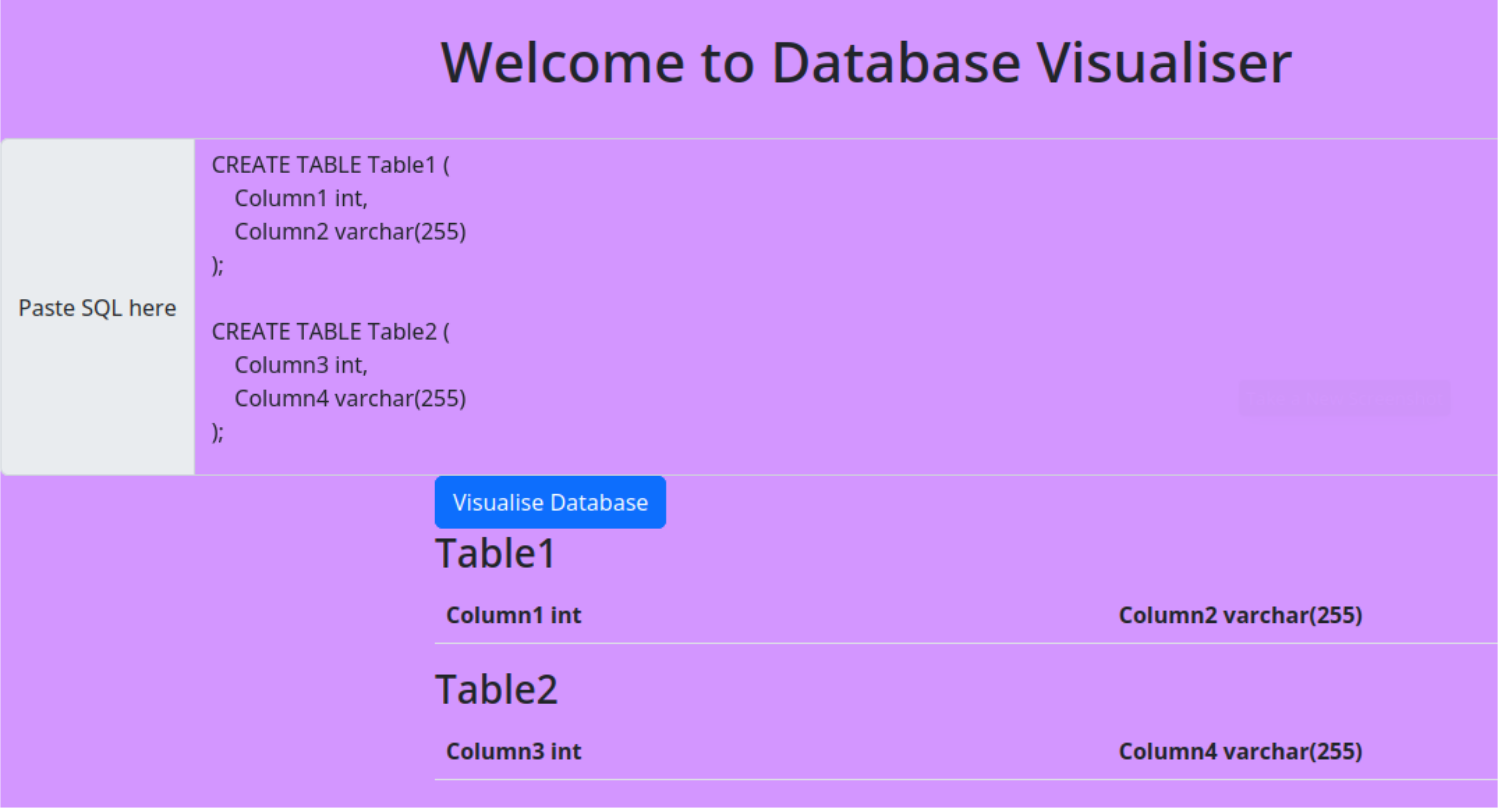
\includegraphics[width=\textwidth]{firstDesign}
	\caption{First iteration of the user interface design}
	\label{fig:firstDesign}
\end{figure}

The first iteration of the design included only the text input in the form with crude parsing of the SQL. The tables are also stretched across the page without borders and styling, and have the column name and data type as columns in the HTML table which might also be confusing.

\newpage

\begin{figure}[h!]
	\centering
	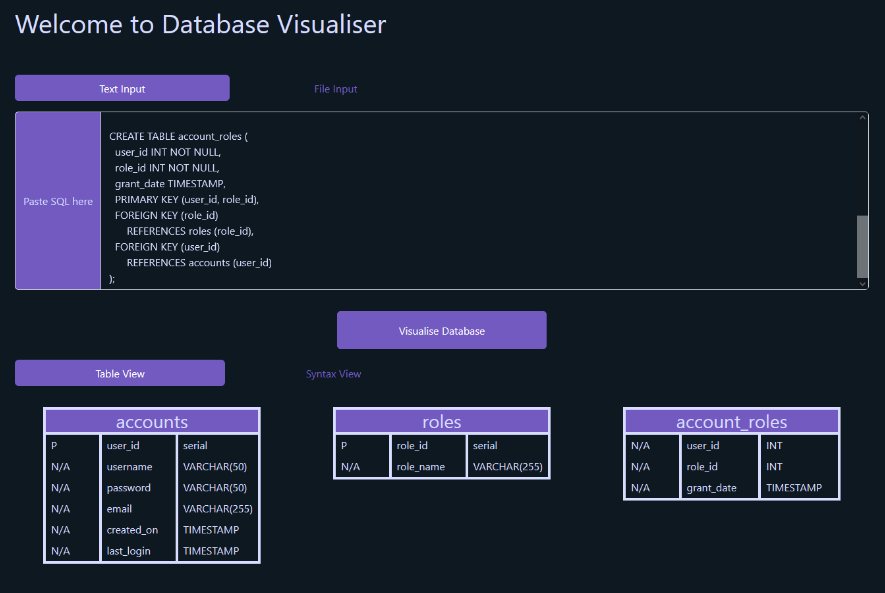
\includegraphics[width=\textwidth]{secondDesign}
	\caption{Second iteration of the user interface design}
	\label{fig:secondDesign}
\end{figure}

The second iteration of the design had a much better colour scheme following the website trend of having a dark background with white text and accent colours. It now also includes the file input tab and the output tabs below the visualise button. However the foreign key arrows have not been implemented yet and the tables here are visualised in the order that they are defined in the SQL file. Also the primary key icons are not yet added and instead are represented as either a "P" for this column being part of a primary key constraint and "N/A" for not having a primary key constraint.

\newpage

\begin{figure}[h!]
	\centering
	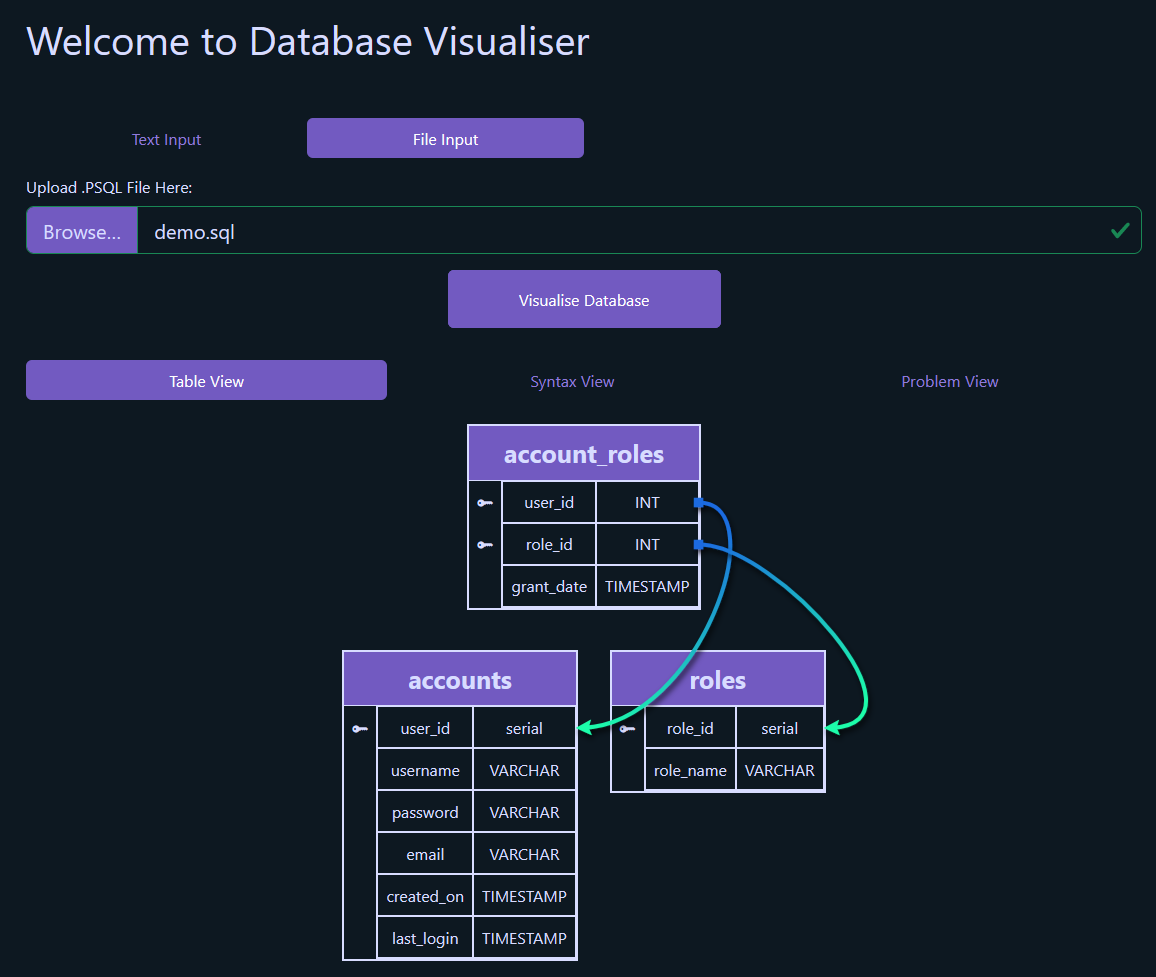
\includegraphics[width=\textwidth]{finalDesign}
	\caption{Final iteration of the user interface design}
	\label{fig:finalDesign}
\end{figure}

The final design builds from the second iteration by adding the tree node structure lay out to tables and the foreign key links between them. The tables are now HTML tables and not the Bootstrap tables made out of row and columns div elements which makes them look slightly more compact and more professional. There are now key icons for the primary key column in each table for the columns that are part of the primary key constraint. It also includes the green outline and tick icon for the input form that is shown when the SQL in the input file, is valid and compiles. The colour scheme has stayed the same since it has not interfered with any of the other elements and did not need to be changed. 